\section{Methodology: The \texttt{FreqDuet} Architecture}
\label{sec:method}

Figure~\ref{fig:architecture} illustrates the closed-loop \texttt{FreqDuet} framework. The architecture comprises four tightly integrated modules: (i) a causal headway-normalized APC rate feed and online Harmonic-RLS frequency decomposer with persistent shock promotion; (ii) an upper slow-clock ($\Delta T_U = 900\text{ s}$) Ensemble SAC planner with exact daily quota conservation; (iii) a causal FIFO Turnaround Budget Ledger updated every $60\text{ s}$; and (iv) a lower stop-event Constrained Ensemble SAC controller equipped with hard turnaround action masking and a zero-hold-advantage critic.

\begin{figure}[t]
  \centering
  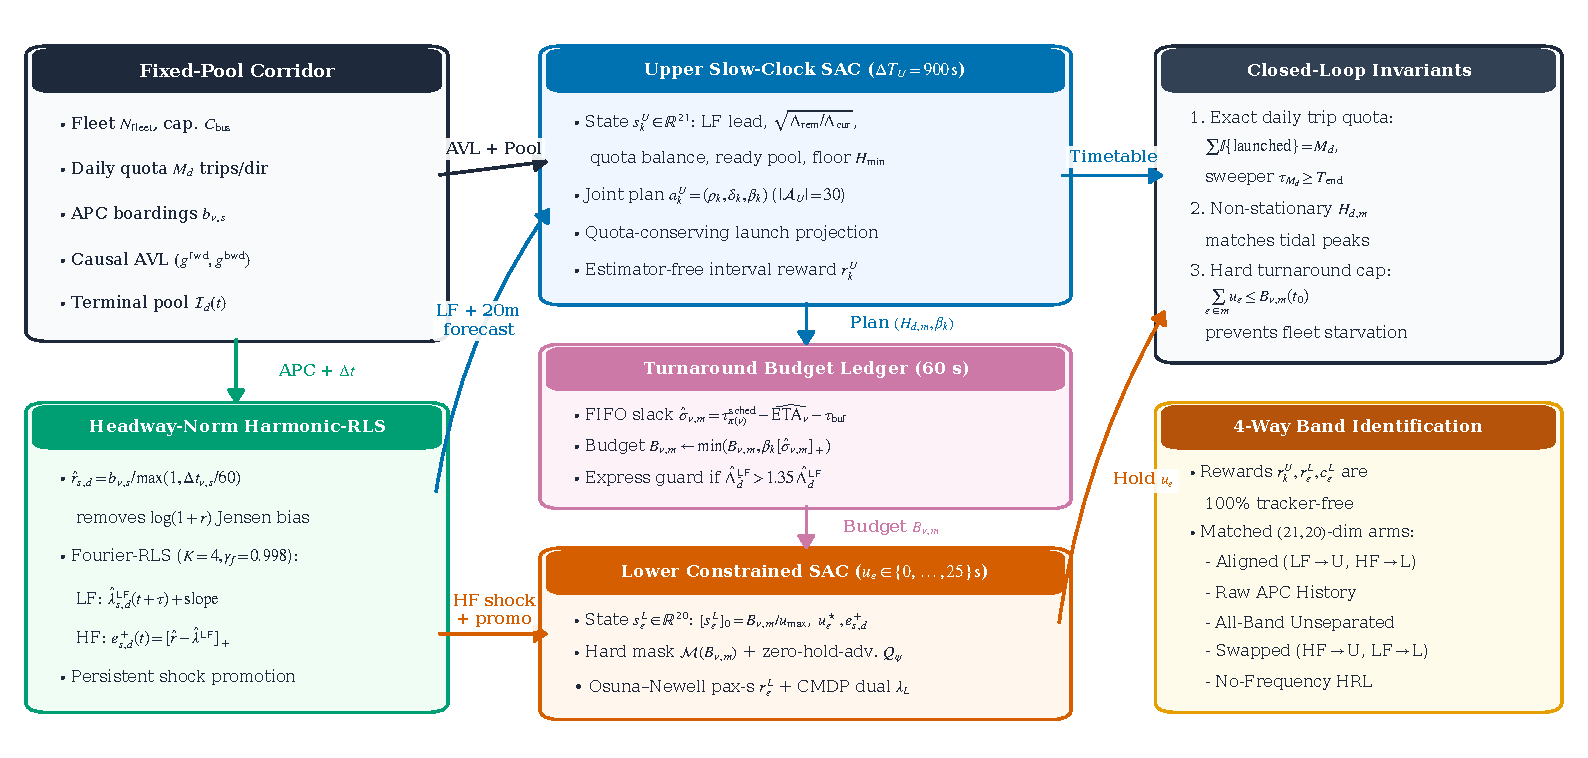
\includegraphics[width=\textwidth]{figures/fig1_architecture.pdf}
  \caption{Overview of the \texttt{FreqDuet} bi-level frequency-separated and turnaround-budgeted constrained reinforcement learning architecture. Low-frequency diurnal level, slope, and $20\text{-min}$ harmonic forecasts guide global quota-conserving timetable allocation, while localized high-frequency positive innovations guide stop-event holding within a hard FIFO turnaround slack budget.}
  \label{fig:architecture}
\end{figure}

\subsection{Causal Headway-Normalized APC Decomposition and Shock Promotion}
\label{sec:method_frequency}

In deployable APC/AVL systems, stop-level passenger demand is not observed continuously; rather, boarding count $b_{v,s}$ is recorded only when vehicle $v$ completes service at stop $(s,d)$ at time $t_e$. If headways average $6\text{ min}$ and raw $1\text{-min}$ APC bins $[0,0,0,0,0,b_{v,s}]$ are fed directly into a concave log-rate filter $y_t = \log(1 + r_t)$, Jensen's inequality ($\frac{1}{6}\log(1 + 6\lambda) \ll \log(1 + \lambda)$) depresses the estimated low-frequency arrival rate by more than $3\times$ (Figure~\ref{fig:corridors}c). Moreover, on the first vehicle visit to stop $(s,d)$ at $t_e$, passengers have accumulated since service opening $t = 0$, not over a nominal headway.

To obtain an unbiased, strictly causal arrival-rate stream, \texttt{FreqDuet} computes the \emph{headway-normalized causal APC rate} upon each boarding completion event $e = (v, s, d, t_e)$:
\begin{equation}
  \begin{aligned}
  \Delta t_e &=
  \begin{cases}
    \mathrm{clip}(h^{\mathrm{arr}}_e,\, 60,\, 1800), & \text{if } (s,d) \text{ has a prior arrival event}, \\
    \mathrm{clip}(\max(60,\, t_e),\, 60,\, 1800), & \text{on the first daily visit to } (s,d),
  \end{cases} \\
  \tilde{b}_e &= b_{v,s} \bigl(1 + 0.15\,\mathbb{I}\{L^{\mathrm{on}}_e = C_{\mathrm{bus}}\}\bigr),
  \end{aligned}
  \label{eq:apc_headway_norm}
\end{equation}
where $h^{\mathrm{arr}}_e$ is the realized arrival headway at $(s,d)$ and the factor $1.15$ provides a conservative causal censoring correction when the departing vehicle reaches full capacity $C_{\mathrm{bus}}$. The instantaneous rate $r^{\mathrm{inst}}_e = 60\,\tilde{b}_e / \Delta t_e$ ($\text{pax/min}$) updates the held stop rate via causal exponential smoothing $\hat{r}_{s,d}(t_e) \leftarrow 0.75\,r^{\mathrm{inst}}_e + 0.25\,\hat{r}_{s,d}(t_e^-)$, which is sampled at $1\text{-min}$ bin closures $n = \lfloor t / 60 \rfloor$.

At each $1\text{-min}$ bin $n$, an online damped Fourier Recursive Least Squares (Harmonic-RLS) estimator models log-intensity $y_{s,d}[n] = \log(1 + \hat{r}_{s,d}[n])$ over harmonic basis $\phi(n) \in \mathbb{R}^{2K+1}$ ($K = 4$, fundamental period $P = 50{,}400\text{ s}$):
\begin{equation}
  \phi(n) = \bigl[1,\, \cos(\omega n),\, \sin(\omega n),\, \dots,\, \cos(K\omega n),\, \sin(K\omega n)\bigr]^\top,
  \qquad
  \omega = \frac{2\pi \cdot 60}{P}.
  \label{eq:fourier_basis}
\end{equation}
Initialized from historical diurnal prior $(\theta_{s,d}[0], P_{s,d}[0] = \sigma_0^2 I)$ with $\sigma_0^2 = 0.35$ and forgetting factor $\gamma_f = 0.998$, the parameter vector updates causally via
\begin{equation}
  \kappa_{s,d}[n] = \frac{P_{s,d}[n-1]\phi(n)}{\gamma_f + \phi(n)^\top P_{s,d}[n-1]\phi(n)},
  \quad
  \theta_{s,d}[n] = \theta_{s,d}[n-1] + \kappa_{s,d}[n]\bigl(y_{s,d}[n] - \phi(n)^\top \theta_{s,d}[n-1]\bigr),
  \label{eq:rls_update}
\end{equation}
with $P_{s,d}[n] = \gamma_f^{-1}(I - \kappa_{s,d}[n]\phi(n)^\top)P_{s,d}[n-1]$. Inverting the log-link yields the causal low-frequency rate $\hat{\lambda}^{\mathrm{LF}}_{s,d}[n] = [\exp(\phi(n)^\top \theta_{s,d}[n]) - 1]_+$, the $\tau$-bin causal forecast $\hat{\lambda}^{\mathrm{LF}}_{s,d}[n+\tau] = [\exp(\phi(n+\tau)^\top \theta_{s,d}[n]) - 1]_+$ ($\tau = 20\text{ min}$), the instantaneous LF slope $\dot{\hat{\lambda}}^{\mathrm{LF}}_{s,d}[n]$, and the high-frequency positive shock residual and shock energy:
\begin{equation}
  e^{+}_{s,d}[n] = \bigl[\hat{r}_{s,d}[n] - \hat{\lambda}^{\mathrm{LF}}_{s,d}[n]\bigr]_+,
  \qquad
  E^{\mathrm{HF}}_{s,d}[n] = (1 - \alpha_E) E^{\mathrm{HF}}_{s,d}[n-1] + \alpha_E \bigl(\hat{r}_{s,d}[n] - \hat{\lambda}^{\mathrm{LF}}_{s,d}[n]\bigr)^2.
  \label{eq:hf_residual}
\end{equation}
Finally, a \emph{persistent shock promotion gate} distinguishes transient $1$--$2\text{ bus}$ boarding bursts from sustained regime shifts (such as unscheduled $1\text{-h}$ peak shifts). Only when $e^{+}_{s,d}$ exceeds $1.25$ standard deviations across at least $55\%$ of a trailing $10\text{-min}$ window (subject to a $15\text{-min}$ cooldown) does the tracker apply an accelerated gain ($\eta_{\mathrm{promo}} = 0.16$) to promote the persistent residual into the LF level $\hat{\lambda}^{\mathrm{LF}}_{s,d}$, while passing a normalized promotion age indicator to the lower controller.

\subsection{Upper Slow-Clock Quota-Conserving Ensemble SAC}
\label{sec:method_upper}

At slow-clock epochs $t_k = k \Delta T_U$ ($\Delta T_U = 900\text{ s}$), the upper controller observes a $21$-dimensional state vector $s^U_k = [x^{\mathrm{ops}}_k;\, z^{\mathrm{U}}_k] \in \mathbb{R}^{21}$. The $13$-dimensional operational core $x^{\mathrm{ops}}_k$ encodes diurnal phase $(\sin\varphi_k, \cos\varphi_k)$, remaining day fraction, directional remaining trip-quota balances, remaining quota-available headways $(H^{\mathrm{avail}}_+, H^{\mathrm{avail}}_-)$, normalized terminal ready counts $(|\mathcal{I}_+|/N_{\mathrm{fleet}}, |\mathcal{I}_-|/N_{\mathrm{fleet}})$, active on-route fleet fraction, dynamic cycle floor $H_{\min}(t_k)$, recent holding budget utilization, and realized readiness delay from the preceding $900\text{ s}$ interval. Under \texttt{FreqDuet}'s aligned routing, the $8$-dimensional demand block $z^{\mathrm{U}}_k$ supplies directional LF current rates, $20\text{-min}$ lead LF rates $\hat{\Lambda}^{\mathrm{LF}}_d = 0.3\sum_s \hat{\lambda}^{\mathrm{LF}}_{s,d}[n] + 0.7\sum_s \hat{\lambda}^{\mathrm{LF}}_{s,d}[n+20]$, directional LF slopes, Newell's root-intensity ratio $\mathbb{E}_{n'>n}[\sqrt{\hat{\Lambda}^{\mathrm{LF}}[n']}]/\sqrt{\hat{\Lambda}^{\mathrm{LF}}[n]}$ \citep{newell1971dispatching}, and directional LF tidal asymmetry $(\hat{\Lambda}^{\mathrm{LF}}_+ - \hat{\Lambda}^{\mathrm{LF}}_-)/(\hat{\Lambda}^{\mathrm{LF}}_+ + \hat{\Lambda}^{\mathrm{LF}}_-)$.

The upper policy $\pi_\theta(a^U_k \mid s^U_k)$ selects from $|\mathcal{A}_U| = 30$ discrete joint plans $a^U_k = (\rho_k, \delta_k, \beta_k)$ formed by the Cartesian product of loop headway compression factor $\rho_k \in \{0.78, 0.89, 1.00, 1.12, 1.24\}$, directional headway tilt $\delta_k \in \{-36, 0, +36\}\text{ s}$, and turnaround budget retention ratio $\beta_k \in \{0.50, 0.90\}$. Desired active-window headways incorporate an inventory guard $g_d(t_k) = \mathrm{clip}(0.55 + 0.35(|\mathcal{I}_d(t_k)| - |\mathcal{I}_{\bar{d}}(t_k)|),\, 0.15,\, 1)$ that suppresses aggressive directional tilting when terminal vehicle stock is depleted:
\begin{equation}
  H^{\mathrm{des}}_d(t_k) = \mathrm{clip}\!\Bigl(H^{\mathrm{avail}}_d(t_k)\,\rho_k + \mathrm{sgn}(d)\,\delta_k\,g_d(t_k),\, H_{\min}(t_k),\, H_{\max}\Bigr),
  \label{eq:desired_headway}
\end{equation}
where $H_{\min}(t_k)$ relaxes down to $0.85\,(\tilde{T}^{\mathrm{run}}_+ + \tilde{T}^{\mathrm{run}}_- + 40)/N_{\mathrm{fleet}}$ when terminal buffer stock $|\mathcal{I}_+| + |\mathcal{I}_-| \ge 3$ and tightens to $0.97$ of steady-state cycle headway when $|\mathcal{I}_+| + |\mathcal{I}_-| \le 1$.

To project $H^{\mathrm{des}}_d(t_k)$ onto the $K^{\mathrm{rem}}_d$ unlaunched mutable trips without violating Eq.~\eqref{eq:quota_sweeper_invariants}, let $\tau^{\mathrm{anc}}_d$ denote the last committed launch time and $S^{\mathrm{rem}}_d = \max(\tau^{\mathrm{base}}_{d,M_d}, T_{\mathrm{end}}) - \tau^{\mathrm{anc}}_d$ the remaining service span. Partitioning $K^{\mathrm{rem}}_d = K^{\mathrm{win}}_d + K^{\mathrm{tail}}_d$ into $K^{\mathrm{win}}_d = \min(K^{\mathrm{rem}}_d - 1, \max(2, \mathrm{round}(W_{\mathrm{act}}/H^{\mathrm{des}}_d)))$ near-term trips ($W_{\mathrm{act}} = 1800\text{ s}$) and $K^{\mathrm{tail}}_d$ tail trips with capacity-safe tail bounds $[T_{\min}, T_{\max}] = [255, 445]\text{ s}$, the executable active headway $H^{\mathrm{act}}_d$ and compensating tail headway $H^{\mathrm{tail}}_d$ are computed in closed form:
\begin{equation}
  \begin{aligned}
  H^{\mathrm{lo}}_d &= \max\!\Bigl(H_{\min},\, \frac{S^{\mathrm{rem}}_d - K^{\mathrm{tail}}_d T_{\max}}{K^{\mathrm{win}}_d},\, t_k + 1 - \tau^{\mathrm{anc}}_d\Bigr), \quad
  H^{\mathrm{hi}}_d = \min\!\Bigl(H_{\max},\, \frac{S^{\mathrm{rem}}_d - K^{\mathrm{tail}}_d T_{\min}}{K^{\mathrm{win}}_d}\Bigr), \\
  H^{\mathrm{act}}_d &= \mathrm{clip}\bigl(H^{\mathrm{des}}_d,\, H^{\mathrm{lo}}_d,\, H^{\mathrm{hi}}_d\bigr), \qquad
  H^{\mathrm{tail}}_d = \frac{S^{\mathrm{rem}}_d - K^{\mathrm{win}}_d H^{\mathrm{act}}_d}{K^{\mathrm{tail}}_d},
  \end{aligned}
  \label{eq:quota_projection}
\end{equation}
with uniform span fallback $H^{\mathrm{act}}_d = H^{\mathrm{tail}}_d = \max(T_{\min}, S^{\mathrm{rem}}_d / K^{\mathrm{rem}}_d)$ whenever $H^{\mathrm{lo}}_d > H^{\mathrm{hi}}_d$, and final sweeper trip $M_d$ pinned to $\max(\tau^{\mathrm{sched}}_{d,M_d-1} + H^{\mathrm{tail}}_d, \max(\tau^{\mathrm{base}}_{d,M_d}, T_{\mathrm{end}}))$.

To resolve long-horizon credit assignment across all $52$ daily slow-clock epochs without biasing the undiscounted passenger journey objective, we introduce a terminal-vanishing potential function $\Phi(s^U_k) = -\sum_{d \in \{+,-\}} \frac{1}{2}\bar{\lambda}_{\mathrm{dir}} S^{\mathrm{rem}}_d(t_k) H^{\mathrm{avail}}_d(t_k)$, where $\bar{\lambda}_{\mathrm{dir}} = P_{\mathrm{prior}}/(2 T_{\mathrm{end}})$ is the static nominal directional arrival rate and $\Phi(s_{\mathrm{term}}) = 0$. Over interval $[t_k, t_{k+1})$, the upper reward is:
\begin{equation}
  \begin{aligned}
  r^U_k &= \frac{-(W^{\mathrm{wait}}_k + W^{\mathrm{hold}}_k) + \gamma_U \Phi(s^U_{k+1}) - \Phi(s^U_k)}{360\,P_{\mathrm{ref}}} \\
        &\quad - 0.08\,\frac{\mathrm{clip}(\mathrm{EWT}_k, -20, 120)}{60}
               - 0.16\,\frac{\mathrm{clip}(\bar{D}^{\mathrm{ready}}_k, 0, 240)}{60}.
  \end{aligned}
  \label{eq:upper_reward}
\end{equation}
Because $\Phi(s^U_0)$ is policy-invariant and $\Phi(s_{\mathrm{term}}) = 0$, potential shaping preserves exact global optimality while immediately pricing quota depletion: differentiating $\frac{1}{2}\lambda_d(t)\Delta T_U H^{\mathrm{act}}_d - [\Phi(s^U_{k+1}) - \Phi(s^U_k)]$ with respect to $H^{\mathrm{act}}_d$ yields the first-order condition $H^{\mathrm{act},\star}_d(t) = H^{\mathrm{avail}}_d \sqrt{\bar{\lambda}_{\mathrm{dir}}/\lambda_d(t)}$, recovering \citet{newell1971dispatching}'s square-root dispatching law while naturally centering $r^U_k$ around zero. Furthermore, because a dispatched bus requires $35\text{--}75\text{ min}$ to complete a corridor round trip, we train $\{Q^U_{\phi_i}\}_{i=1}^{6}$ ($\gamma_U = 0.996$) using exact $N_U = 6$-step ($90\text{-min}$) Bellman backups with pessimistic LCB targets ($\beta_{\mathrm{LCB}} = -1.0$) \citep{haarnoja2018soft,christodoulou2019discrete,chen2021redq}.

\subsection{Causal Turnaround Budget Ledger}
\label{sec:method_ledger}

Every $60\text{ s}$ and upon any vehicle launch, the \emph{Turnaround Budget Ledger} translates the active timetable and upper retention tier $\beta_k \in \{0.50, 0.90\}$ into per-trip remaining holding budgets $B_{v,m}(t)$ without future oracle knowledge. For each direction $\bar{d}$, the ledger constructs the causal supply set of vehicles that will feed terminal $s_{\bar{d},0}$: (i) vehicles already idle at $s_{\bar{d},0}$ with ready time $\max(t, \tau^{\mathrm{ret}}_v + 1)$, and (ii) vehicles currently en route in direction $d$ at normalized corridor progress $\tilde{p}_v = d^{\mathrm{trav}}_v / L_d \in [0, 1]$, whose causal opposite-terminal ready ETA is
\begin{equation}
  \widehat{\mathrm{ETA}}_v(t) = t + (1 - \tilde{p}_v)\,\tilde{T}^{\mathrm{run}}_d(t) + h^{\mathrm{rem}}_v + w^{\mathrm{rem}}_v + 1,
  \label{eq:ledger_eta}
\end{equation}
where $h^{\mathrm{rem}}_v$ and $w^{\mathrm{rem}}_v$ are residual in-progress stop holding and dwell times. Sorting the supply set by $\widehat{\mathrm{ETA}}_v(t)$ and matching it in FIFO order against the sorted unlaunched schedule $\{\tau^{\mathrm{sched}}_{\bar{d},m'}\}$ assigns each active en-route trip $(v,m)$ to its paired opposite-direction launch $\pi(v,m)$ with projected turnaround slack $\hat{\sigma}_{v,m}(t) = \tau^{\mathrm{sched}}_{\pi(v,m)} - \widehat{\mathrm{ETA}}_v(t) - \tau_{\mathrm{buf}}$ ($\tau_{\mathrm{buf}} = 20\text{ s}$).

To prevent deadheading starvation during sharp tidal asymmetries, when opposite-direction LF demand dominates own-direction LF demand ($\hat{\Lambda}^{\mathrm{LF}}_{\bar{d}} > 1.35\,\hat{\Lambda}^{\mathrm{LF}}_d$) and $\hat{\sigma}_{v,m}(t) < 75\text{ s}$, the ledger activates a \emph{backhaul express guard}, tightening the proposed budget cap:
\begin{equation}
  B^{\mathrm{prop}}_{v,m}(t) =
  \begin{cases}
    \mathrm{clip}\bigl(0.40\,\beta_k\,[\hat{\sigma}_{v,m}(t)]_+,\, 0,\, 30\text{ s}\bigr), & \text{if } \hat{\Lambda}^{\mathrm{LF}}_{\bar{d}} > 1.35\,\hat{\Lambda}^{\mathrm{LF}}_d \text{ and } \hat{\sigma}_{v,m}(t) < 75\text{ s}, \\
    \mathrm{clip}\bigl(\beta_k\,[\hat{\sigma}_{v,m}(t)]_+,\, 0,\, 85\text{ s}\bigr), & \text{otherwise}.
  \end{cases}
  \label{eq:budget_proposal}
\end{equation}
Remaining trip budget updates monotonically via $B_{v,m}(t) \leftarrow \min(B_{v,m}(t^-),\, B^{\mathrm{prop}}_{v,m}(t))$ and is debited immediately upon every stop-level hold: $B_{v,m}(t^+) \leftarrow \max(0,\, B_{v,m}(t) - u_e)$. Thus cumulative holding along trip $(v,m)$ can never exceed available turnaround slack.

\subsection{Lower Hard-Masked Zero-Hold-Advantage Constrained SAC}
\label{sec:method_lower}

Whenever vehicle $v$ finishes passenger boarding at intermediate stop $s \in \{1, \dots, S_d-1\}$, the lower agent observes a $20$-dimensional state $s^L_e = [x^{\mathrm{loc}}_e;\, z^{\mathrm{L}}_e] \in \mathbb{R}^{20}$ and selects a discrete holding duration $u_e \in \mathcal{A}_L = \{0, 5, 10, 15, 20, 25\}\text{ s}$ ($u_{\max} = 25\text{ s}$). Critically, feature zero is defined as the normalized budget limit ratio $[s^L_e]_0 = \min(u_{\max}, B_{v,m}(t_e)) / u_{\max} \in [0, 1]$, followed by $15$ causal operational features (remaining trip budget, per-remaining-stop budget allowance, turnaround slack $\hat{\sigma}_{v,m}$, opposite-terminal overdue launch indicator, relative forward and backward gaps $(g^{\mathrm{fwd}} - H_{\mathrm{own}})/H_{\mathrm{own}}$ and $(g^{\mathrm{bwd}} - H_{\mathrm{fol}})/H_{\mathrm{fol}}$, two-sided AVL validity flag, analytical plan-consistent target $u^\star_e / u_{\max}$ from Proposition~\ref{prop:nonstationary_target}, own and follower planned headways, onboard load ratio $L^{\mathrm{on}}_e/C_{\mathrm{bus}}$, pass-up count, route progress, and diurnal phase). Under aligned frequency routing, the $4$-dimensional band block $z^{\mathrm{L}}_e$ supplies normalized local HF shock $e^{+}_{s,d}/\max(\hat{\lambda}^{\mathrm{LF}}_{s,d}, 0.5)$, local HF shock RMS $\sqrt{E^{\mathrm{HF}}_{s,d}}/\max(\hat{\lambda}^{\mathrm{LF}}_{s,d}, 0.5)$, maximum HF shock over the next two downstream stops, and local promotion age.

Three structural mechanisms stabilize lower-level learning across hundreds of training episodes:
\begin{enumerate}
  \item \textbf{Differentiable hard budget masking:} Directly inside the categorical policy network $\pi_\omega(u \mid s^L_e)$, action logits $\ell_\omega(s^L_e, u)$ for any bin $u > [s^L_e]_0 \cdot u_{\max}$ are masked to $-\infty$ during both rollout sampling and Bellman target evaluation:
  \begin{equation}
    \pi_\omega(u \mid s^L_e) = \frac{\exp(\ell_\omega(s^L_e, u))\,\mathbb{I}\{u \le B_{v,m}(t_e)\}}{\sum_{u' \in \mathcal{A}_L} \exp(\ell_\omega(s^L_e, u'))\,\mathbb{I}\{u' \le B_{v,m}(t_e)\}},
    \label{eq:hard_action_mask}
  \end{equation}
  where $u = 0$ is always feasible. Because $[s^L_e]_0$ is stored in every replay transition, target-policy backups at $s^L_{e'}$ automatically respect the exact physical budget active at the next stop.

  \item \textbf{Zero-hold-advantage ensemble critic:} Each of the $E = 6$ reward critics is parameterized as a dueling zero-hold-anchored decomposition:
  \begin{equation}
    Q^L_{\psi_i}(s^L_e, u) = V_{\psi_i}(s^L_e) + \mathbb{I}\{u > 0\}\,A_{\psi_i}(s^L_e, u), \qquad u \in \mathcal{A}_L.
    \label{eq:zero_hold_advantage}
  \end{equation}
  Because $Q^L_{\psi_i}(s^L_e, 0) \equiv V_{\psi_i}(s^L_e)$ identically, $A_{\psi_i}(s^L_e, u)$ directly represents the marginal person-seconds advantage of holding $u > 0$ over immediate departure ($u = 0$), eliminating shared-baseline drift across discrete bins.

  \item \textbf{Estimator-free Osuna--Newell reward and CMDP Lagrangian safety dual:} Following Proposition~\ref{prop:osuna_turnaround}, upon trip completion at the receiving terminal, each stop decision $e$ along trip $(v,m)$ settles using the exact realized downstream passenger arrival rate $\Lambda^{\mathrm{ds}}_e = \sum_{s' > s} b_{v,s'}/\mathrm{clip}(h^{\mathrm{arr}}_{v,s'}, 90, 900)$ across all remaining stops of that trip (with $\Lambda^{\mathrm{ds}}_e \equiv 0$ at the final intermediate stop), without referencing the frequency tracker:
  \begin{align}
    r^L_e &= \mathrm{clip}\!\left(\frac{\Delta W_{\mathrm{save}}(u_e) - L^{\mathrm{on}}_e u_e - \phi_{\mathrm{slack}}(\hat{\sigma}_{v,m}, u_e)}{150},\, -2.5,\, 2.5\right), \quad r^L_e(u_e=0) = 0, \label{eq:lower_reward} \\
    c^L_e &= \min\!\Bigl(8\,\bigl[\mathcal{L}_{\mathrm{reg}}(u_e) - \mathcal{L}_{\mathrm{reg}}(0)\bigr]_+ \nonumber \\
          &\qquad\quad + \bigl(0.25\,[L^{\mathrm{on}}_e/C_{\mathrm{bus}} - 0.55]_+ + 0.35\,\mathbb{I}\{\hat{\sigma}_{v,m} < 15\}\bigr)\frac{u_e}{u_{\max}},\, 2.0\Bigr), \label{eq:lower_cost}
  \end{align}
  where $\phi_{\mathrm{slack}}$ penalizes tight-slack and terminal-deficit holding. A separate cost critic $Q^C_\xi(s^L_e, u)$ estimates discounted constraint cost, and a non-negative Lagrange multiplier $\lambda_L = \exp(\eta_L)$ updates via dual ascent to enforce $\mathbb{E}_\pi[Q^C_\xi(s^L, u)] \le d_0 = 0.020$ \citep{altman1999constrained,stooke2020responsive}, yielding the actor loss:
  \begin{equation}
    \mathcal{J}_\pi(\omega) = \mathbb{E}_{s^L \sim \mathcal{D}_L}\!\Biggl[\sum_{u \in \mathcal{M}(s^L)} \pi_\omega(u \mid s^L)\Bigl(\alpha_L \log \pi_\omega(u \mid s^L) - Q^L_{\mathrm{LCB}}(s^L, u) + \lambda_L Q^C_\xi(s^L, u)\Bigr)\Biggr].
    \label{eq:lower_actor_loss}
  \end{equation}
\end{enumerate}

Algorithm~\ref{alg:freqduet} summarizes the complete online execution and bi-level off-policy training procedure.

\begin{algorithm}[t]
\caption{\texttt{FreqDuet}: Frequency-Separated Turnaround-Budgeted Bi-Level Constrained SAC}
\label{alg:freqduet}
\footnotesize
\begin{algorithmic}[1]
\Require Fixed fleet $N_{\mathrm{fleet}}$, daily quotas $(M_+, M_-)$, Fourier prior $(\theta[0], \sigma_0^2 I)$, Upper Ensemble SAC $(\pi_\theta, \{Q^U_{\phi_i}\}_{i=1}^6)$, Lower Constrained Ensemble SAC $(\pi_\omega, \{Q^L_{\psi_i}\}_{i=1}^6, Q^C_\xi, \lambda_L)$, replay buffers $(\mathcal{D}_U, \mathcal{D}_L)$.
\For{training episode $n_{\mathrm{ep}} = 1, \dots, N_{\mathrm{ep}}$}
  \State Reset corridor simulation with scenario seed; initialize headway-normalized APC rate feed, Harmonic-RLS, and Turnaround Budget Ledger.
  \While{corridor episode not terminated ($t \le T_{\mathrm{eval}}$)}
    \State Sync newly launched and completed trips in the Turnaround Budget Ledger; push terminal lower transitions to $\mathcal{D}_L$.
    \If{$t \le T_{\mathrm{replan}}$ \textbf{and} $\lfloor t / \Delta T_U \rfloor > k_{\mathrm{prev}}$} \Comment{Slow-clock epoch ($\Delta T_U = 900\text{ s}$)}
      \State Settle preceding interval reward $r^U_{k-1}$ via Eq.~\eqref{eq:upper_reward} and store $(s^U_{k-1}, a^U_{k-1}, r^U_{k-1}, s^U_k)$ in $\mathcal{D}_U$.
      \State Construct $s^U_k \in \mathbb{R}^{21}$ from operational state and LF forecast/slope features; sample $a^U_k = (\rho_k, \delta_k, \beta_k) \sim \pi_\theta(\cdot \mid s^U_k)$.
      \State Project quota-conserving timetable $\{H^{\mathrm{act}}_d, H^{\mathrm{tail}}_d\}$ with sweeper pin via Eqs.~\eqref{eq:desired_headway}--\eqref{eq:quota_projection}.
      \State Set ledger retention $\beta_k$ and refresh FIFO turnaround budgets $\{B_{v,m}(t)\}$ via Eqs.~\eqref{eq:ledger_eta}--\eqref{eq:budget_proposal}.
    \ElsIf{new trip launched \textbf{or} $t - t_{\mathrm{refresh}} \ge 60\text{ s}$}
      \State Refresh FIFO turnaround budgets $\{B_{v,m}(t)\}$ using current directional LF rates.
    \EndIf
    \For{each vehicle $v$ waiting for stop-holding decision $e$ at intermediate stop $(s,d)$}
      \State Settle vehicle $v$'s previous stop reward/cost $(r^L_{e^-}, c^L_{e^-})$ via Eqs.~\eqref{eq:lower_reward}--\eqref{eq:lower_cost}; push transition to $\mathcal{D}_L$.
      \State Build $s^L_e \in \mathbb{R}^{20}$ with $[s^L_e]_0 = \min(u_{\max}, B_{v,m}(t))/u_{\max}$ and local HF shock features $z^{\mathrm{L}}_e$.
      \State Sample feasible hold $u_e \sim \pi_\omega(\cdot \mid s^L_e)$ under hard mask $u_e \le B_{v,m}(t)$ (Eq.~\eqref{eq:hard_action_mask}); debit $B_{v,m} \leftarrow B_{v,m} - u_e$.
    \EndFor
    \State Step physical transit simulator by $1\text{ s}$; update headway-normalized APC rates (Eq.~\eqref{eq:apc_headway_norm}) and $1\text{-min}$ Harmonic-RLS / promotion state (Eqs.~\eqref{eq:rls_update}--\eqref{eq:hf_residual}).
  \EndWhile
  \State Perform $G_U = 32$ Ensemble SAC gradient updates on $(\pi_\theta, \{Q^U_{\phi_i}\}, \alpha_U)$ from $\mathcal{D}_U$ and $G_L = 64$ Constrained Ensemble SAC updates on $(\pi_\omega, \{Q^L_{\psi_i}\}, Q^C_\xi, \alpha_L, \lambda_L)$ from $\mathcal{D}_L$ (Eq.~\eqref{eq:lower_actor_loss}).
\EndFor
\end{algorithmic}
\end{algorithm}
